\chapter{Исследовательский раздел}
В данном разделе произведен ряд экспериментов с полученным, в ходе написания проекта, программным обеспечением.
Для проведения серии экспериментов необходимо подготовить набор тестовых входных данных, представляющих собой тридцать электронных документов на русском языке, формата PDF.
Все работы участвующие в эксперименте взяты с сайта \href{https://cyberleninka.ru/article}{cyberleninka.ru}
Для тестов отбираются тексты с указанными ключевыми словами.
Для удобства анализа, многокомпонентные ключевые слова из документов разбиваются на отдельные термины.

Для обеспечения качества проводимых экспериментов необходимо указать критерии по которым будет производиться отбор документов:
\begin{enumerate}
	\item документ должен содержать в себе текст, а не отсканированные изображения страниц ранее опубликованных работ, поскольку это приводит к невозможности прочтения документа;
	\item информация, содержащаяся в документе должна быть целостной, то есть принадлежать одной работе.
\end{enumerate}

\section{Исследование характеристик метода}
В процессе данного эксперимента ставится задача сравнить модифицированный метод с аналогами, способными на работу с документами на русском языке.
Для этой цели были выбраны следующие алгоритмы:
\begin{enumerate}
	\item Rake;
	\item Textrank.
\end{enumerate}
В качестве тестовых данных использовались тридцать ранее отобранных документов с ключевыми словами.
Исследуется процент от ключевых слов полученных из метода, попавших в пересечение с словами выделенными авторами, так же изучется процент не попавших в пересечение

Для методов были выбраны следующие настройки, отображенные на рисунке \ref{fig:nbarsukov20220605a9e9}
% TODO: \usepackage{graphicx} required
\begin{figure}[!h]
	\centering
	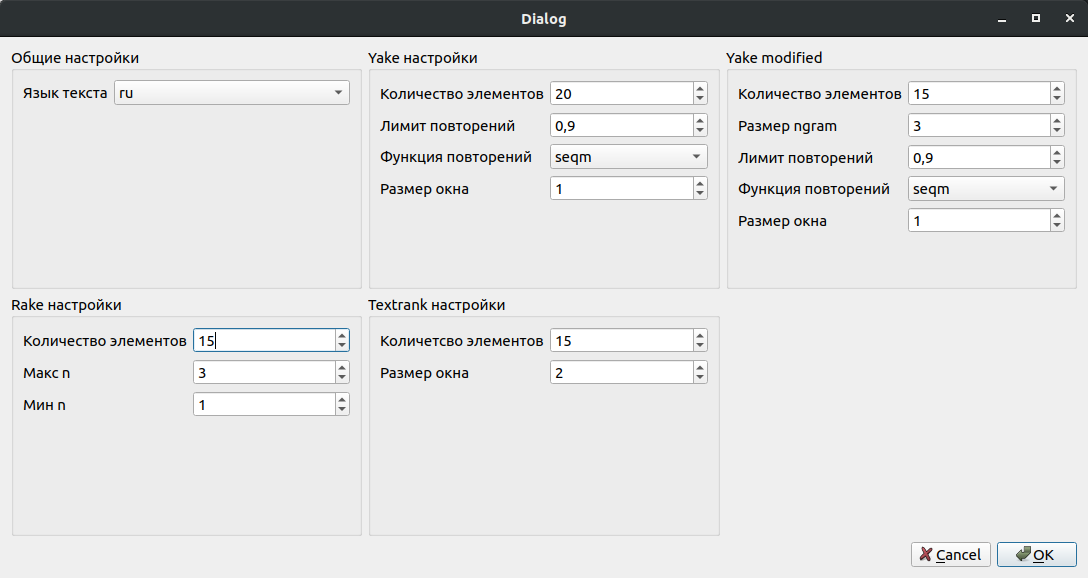
\includegraphics[width=0.9\linewidth]{src/img/experiment/nbarsukov_20220605_a9e9}
	\caption{Настройки методов}
	\label{fig:nbarsukov20220605a9e9}
\end{figure}

% TODO: \usepackage{graphicx} required
\begin{figure}
	\centering
	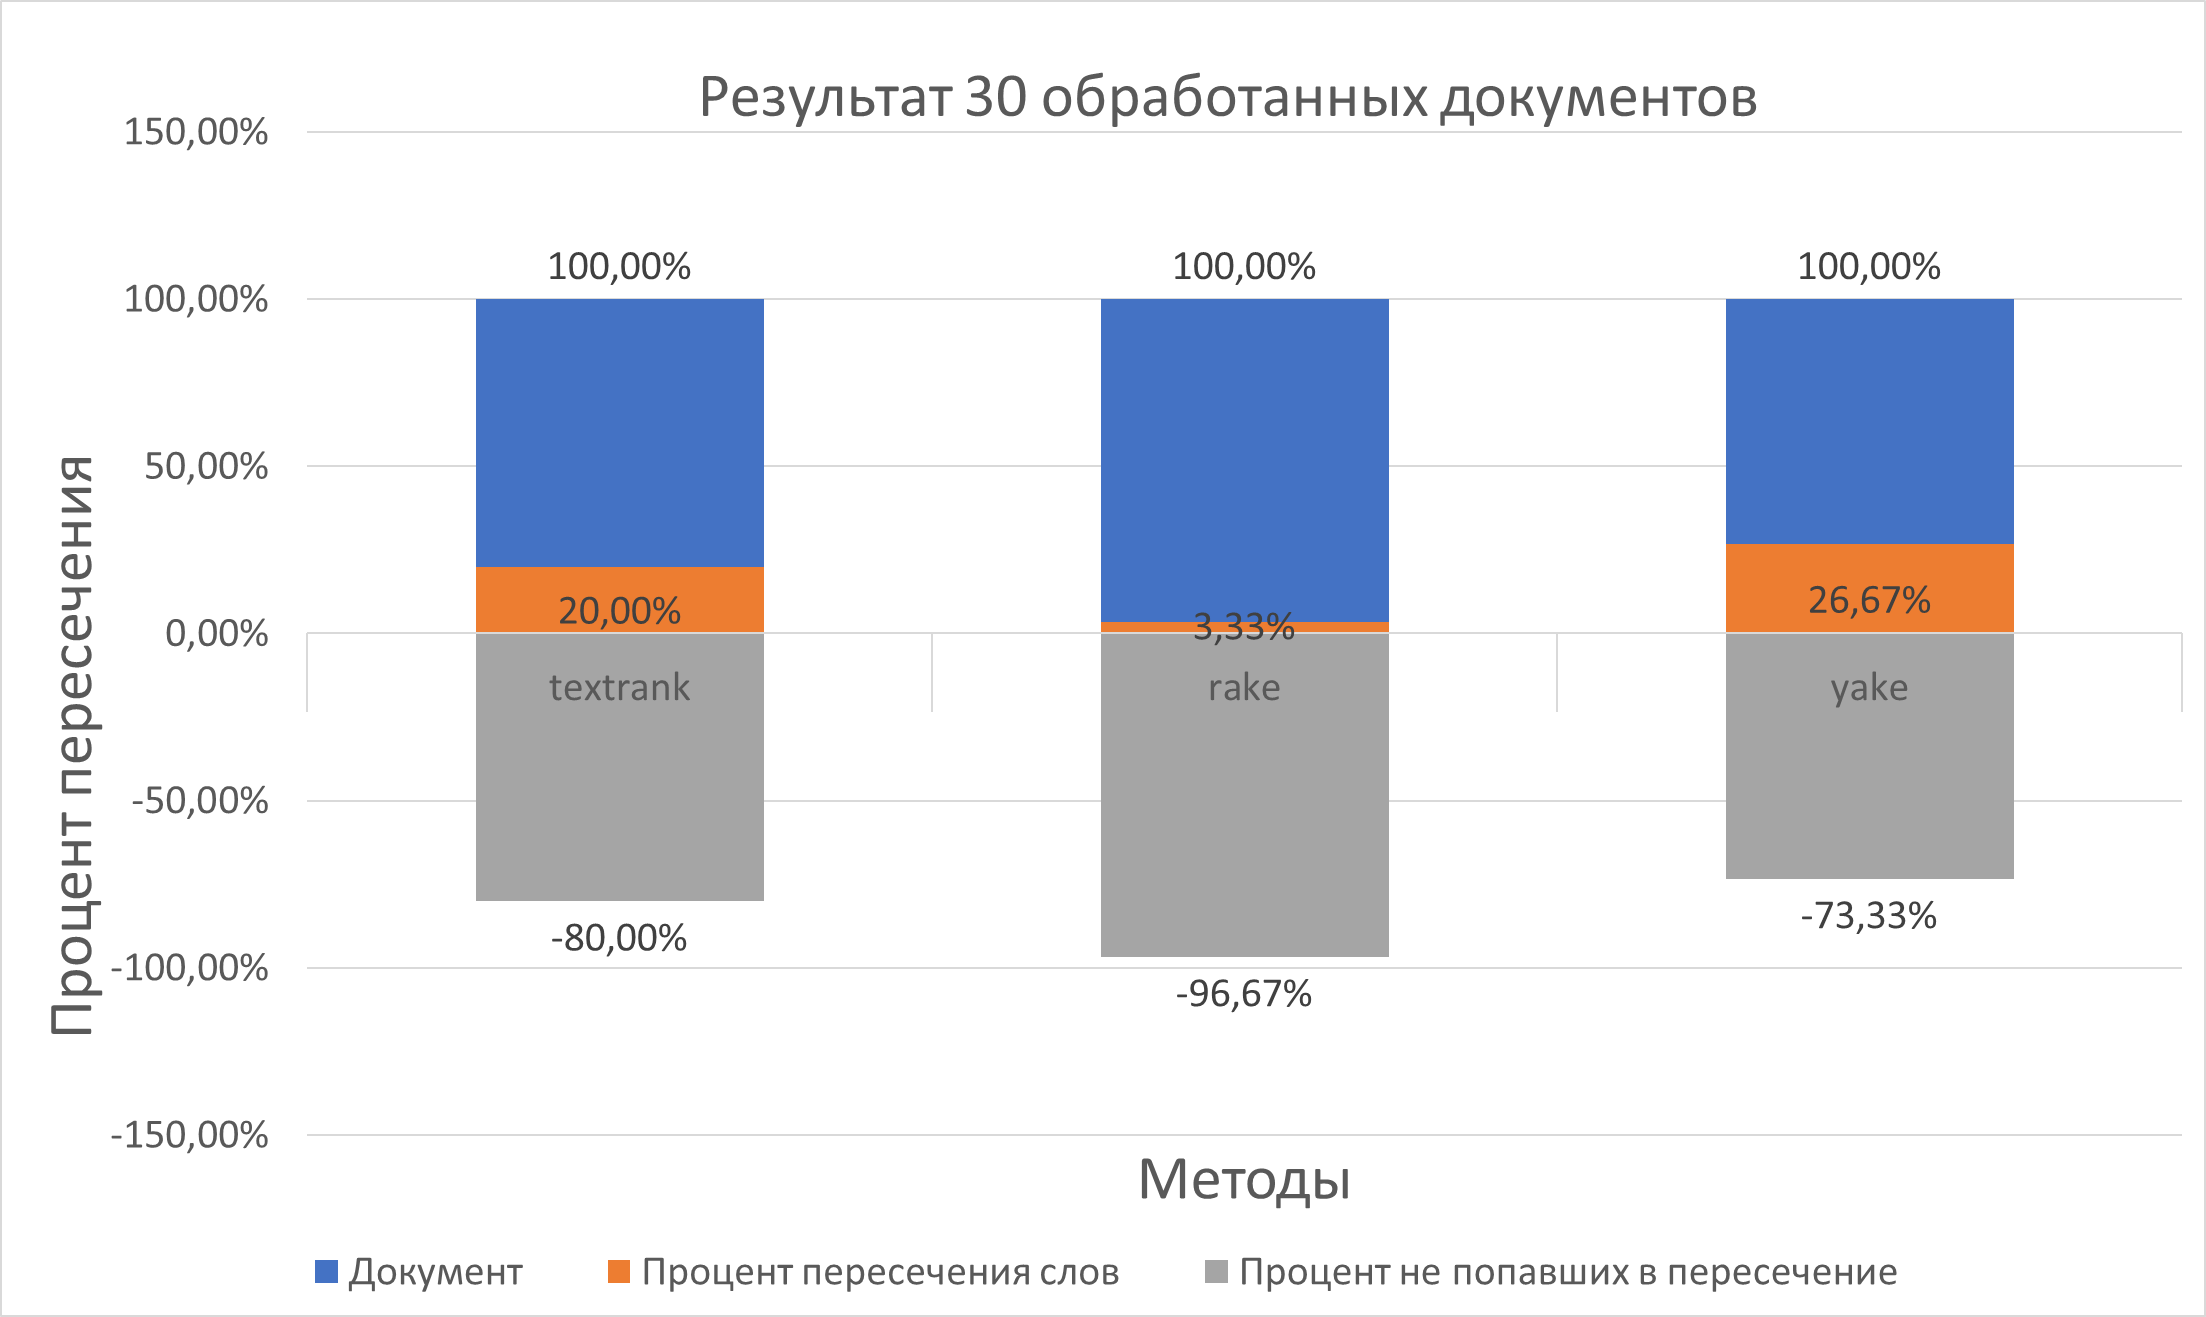
\includegraphics[width=0.7\linewidth]{src/img/experiment/experiment_1_4}
	\caption{Результат обработки 30 документов}
	\label{fig:experiment14}
\end{figure}

По завершению измерений результативности были получены следующие результаты, отображенные в таблице на странице \pageref{table:experiment31}
\begin{table}[!h]
	\begin{tabular}{|c|c|c|c|}
		\hline
		& Yake (mod) & Textrank & Rake \\
		\hline
		Средний \% пересечения & 26.67\% & 20\% & 3.33\% \\
		\hline
		Средний \% не попавших в пересечение & 73.33\% & 80\% & 96.67\% \\
		\hline
	\end{tabular}
	\label{table:experiment31}
	\caption{Результат сравнения методов}
\end{table}
Результатом 30 обработок документа является средний процент пересечения ключевых слов у метода Yake составляет 26.67\% в то время когда у Textrank 20 \% у Rake 3.33%.
Процент ключевых слов не попавших в пересечении у метода Yake составляет 73.33\% у Textrank 80\% а у метода rake составил 96.67\%

\section{Исследование влияния размерности N-грамм на работу метода}
Для проведения данного исследования был выбран документ: "Идентификация личности по фрактальной размерности отпечатков пальцев и системы контроля и управления доступом" \cite{24}.

\begin{figure}[!h]
	\centering
	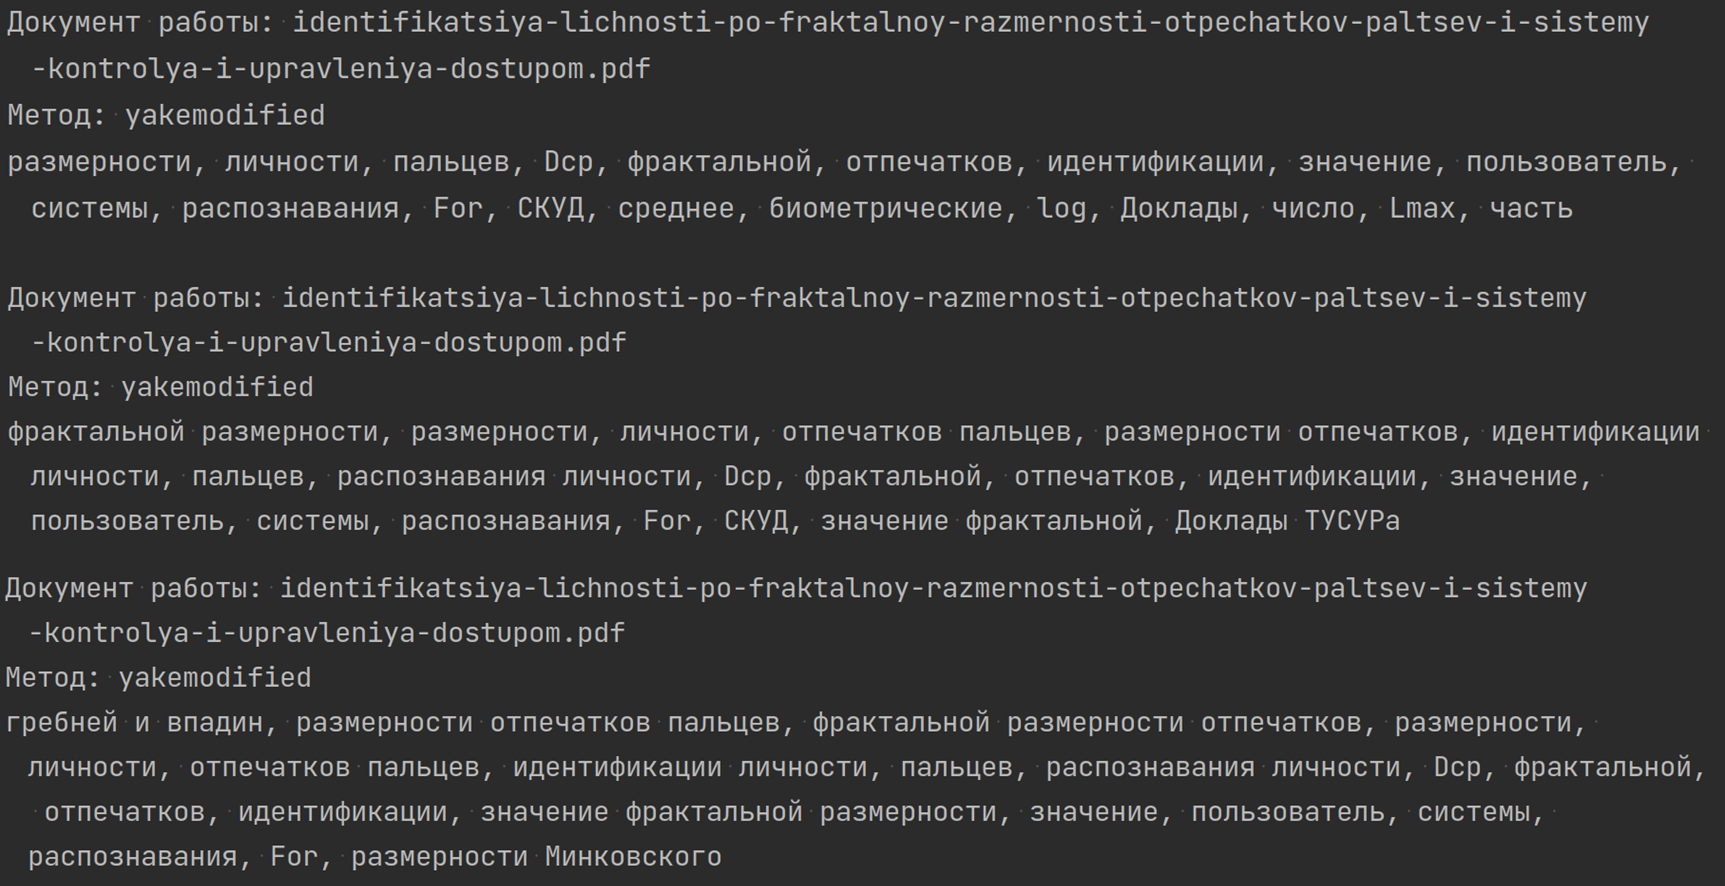
\includegraphics[width=0.9\linewidth]{src/img/experiment/experiment_2_1}
	\caption{Результа извлечения ключевых слов при N = 1 до N = 3}
	\label{fig:experiment21}
\end{figure}

В качестве опорного слова возьмем "пальцев". При N = 2 данное слово преобразуется в словосочетание "отпечатков пальцев". При N = 3 получаем выражением "размерности отпечатков пальцев". На основе этого можно сделать вывод, что метод пригоден для извлечения многокомпонентных ключевых слов.

\section{Вывод}
В результате проведенной исследовательской работы над разработанным решением было установлено, что все требования, поставленные к алгоритму, соблюдены.
Метод способен на извлечение многокомпонентных ключевых слов из документов на русском языке. 
